%%%%%%%%%%%%%%%%%%%%%%%%%%%%%%%%%%%%%%%%%%%%%%%%%%%%%%%%%%%%%%%%%%%%%%%%%%%%%%%
\chapter{Power-aware throughput management on multi-core systems}~\label{chap:delta}
%%%%%%%%%%%%%%%%%%%%%%%%%%%%%%%%%%%%%%%%%%%%%%%%%%%%%%%%%%%%%%%%%%%%%%%%%%%%%%%

Power management systems have to look at two facets: Power and energy. Servers are
usually limited to the amount of peak power and energy
consumed in order to reduce maintenance cost. Power and energy considerations more often than not, accounts 
to the reduction in server space expansion in industries. To combat these constraints, power management systems
are becoming increasingly common in the server space which were previously restricted for mobile devices.
Two common methodologies exist to reduce the power consumption of a compute element. The first among which
is to turn off (and hence reduce the power consumption to the orders of milliwatts) processors during idle time. 
The second is to lower the operating frequency and voltage of the processor at idle or active time to observe
a proportionally lower power consumption.
In order to fully utilize server nodes and minimize idle time, the current trend among industries is to 
run multiple \textit{virtual machines} on a single server rack thus making varied workloads common place
in an otherwise single purpose server usage. This element further enhances the requirement of 
dynamic non-trace driven power management systems. \cite{VirtualPower} discusses a power optimizer specialized
for a virtual machine farm, but fail to recognize the workload characteristics of these systems.

Lowering frequency has a pleasant benefit of reducing the power consumption and hence
the energy and cooling costs. But as shown in Chapter~\ref{chap:pds}, Figures~\ref{fig:ipc_speedup} 
and \ref{fig:ipc_epi}, when the average IPC of an application is high, reduction in 
frequency only causes the application to execute for a proportionally longer duration and 
hence having no energy benefit (Figure~\ref{fig:ipc_epi}). The only advantage of reducing
the frequency is the reduction of energy supply into the system per unit time and hence
possibly lower heat dissipation. 

Some power management systems such as \cite{OnDemand} manipulate the DVFS (dynamic voltage and freqency) configuration
of the system based on the load. The primary problem with such approaches are not in
their implementation or design, but the fact that there are better power management
systems where the entire processor is powered down during idle time whose power savings are considerably higher than DVFS. 
This brings us to utilizing DVFS mechanisms to conserve power during system \textit{active}
state. 

\cite{AnIntraTask}, \cite{LiveRuntime} and \cite{Phaseaware} propose adapting the clock speed of the the processing element based
on the current application's demand. All these methodologies assumes the fact that DVFS transitions
are local to that processor core. Some multi-core processors have dependency between 
processor cores (transitioning one might potentially transition the other) or systems with 
symmetric multi-threaded features where a single processor
core is visible to the operating system as multiple virtual processors. Thus, applications
executing on such processing elements are tied to each other and any DVFS
transition based on one application might potentially affect another negatively. 
Chapter~\ref{chap:pds} showed that such transitions could be remedied with a simple processor migration
requiring power optimizers to react to the needs of a scheduler.

%%%%%%%%%%%%%%%%%%%%%%%%%%%%%%%%%%%%%%%%%%%%%%%%%%%%%%%%%%%%%%%%%%%%%%%%%%%%%%%
\section{Common power management systems}~\label{sec:common_pow}
%%%%%%%%%%%%%%%%%%%%%%%%%%%%%%%%%%%%%%%%%%%%%%%%%%%%%%%%%%%%%%%%%%%%%%%%%%%%%%%

The most popular among power management techniques are load directed systems
which transition a processor to a higher or lower performance state based on it's current load. Two
of these techniques: \textit{ondemand}\cite{OnDemand} and \textit{conservative} 
were simulated within the existing infrastructure. The \textit{ondemand}
system raises the performance state to the highest possible level at high loads, and
reduces the performance state gradually to the lowest state during lower load.
The \textit{conservative}
system gradually changes the performance state in either direction. These two are 
shown in Figures \ref{fig:math_ondemand} and \ref{fig:math_conservative}. As both 
are similar in design, only the \textit{ondemand} system was heavily analyzed 
along with the proposed power management systems.

\begin{figure}[h!]
\centering
\begin{equation*}
    P_{i}' = \left\{ \begin{array}{lr} 
                   P_{M-1} & : Load \geq 0.8 \\
		   P_{i}-1 & : Load < 0.8
                  \end{array} \right.
\end{equation*}
\caption{The ondemand power management system with M performance states}
\label{fig:math_ondemand}
\end{figure}

\begin{figure}[h!]
\centering
\begin{equation*}
    P_{i}' = \left\{ \begin{array}{lr} 
                   P_{i}+1 & : Load \geq 0.8 \\
		   P_{i}-1 & : Load < 0.8
                  \end{array} \right.
\end{equation*}
\caption{The conservative power management system with M performance states}
\label{fig:math_conservative}
\end{figure}

%%%%%%%%%%%%%%%%%%%%%%%%%%%%%%%%%%%%%%%%%%%%%%%%%%%%%%%%%%%%%%%%%%%%%%%%%%%%%%%
\section{Overview of the Linux cpufreq architecture}~\label{sec:cpufreq}
%%%%%%%%%%%%%%%%%%%%%%%%%%%%%%%%%%%%%%%%%%%%%%%%%%%%%%%%%%%%%%%%%%%%%%%%%%%%%%%

In order to maintain architecture independence, separation of methodology 
and policy, the subsystem in the Linux kernel responsible for managing the 
voltage and frequency configuration separates the procedure into three layers. \textit{cpufreq-drivers}
are responsible for the actual P-State transition and register with the 
intermediate \textit{cpufreq} layer. \textit{cpufreq-governors} are responsible for
policy (How and when to initiate a transition) and also register with the 
\textit{cpufreq} layer. Once a working configuration is initialized, the 
\textit{cpufreq-governor} instructs the \textit{cpufreq-driver} in an indirect
fashion on the required transition. As most of the experimentation mentioned in
this text relates to the AMD Barcelona, the \textit{powernow-k8} \textit{cpufreq-driver}
was used to initiate the transition. 

A \textit{cpufreq} governor \textit{seeker}
was developed having kernel exported interfaces for the mutator to request transitions. 
A simple registration method was introduced to allow the mutator to be informed 
every time a transition is complete as shown in Figure~\ref{fig:governor}. 
The asynchronous call back mechanism allows the mutator to
update its data structures even when an entity other than itself ( For example, through
the \textit{sysfs} interface) requests for a performance state change. 

\begin{figure}[h!]
  \begin{center}
    %\resizebox{\columnwidth}{!}{
    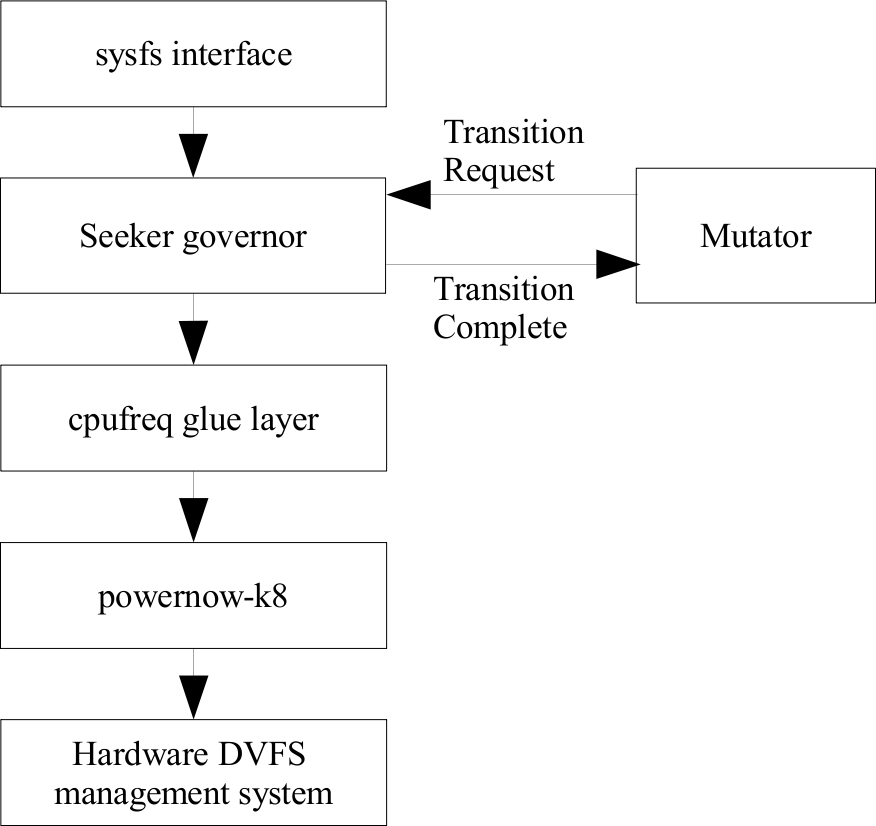
\includegraphics[height=2in]{figures/seeker_governor.jpg}%}
    \caption{The Seeker governor}
    \label{fig:governor}
  \end{center}
\end{figure}

%%%%%%%%%%%%%%%%%%%%%%%%%%%%%%%%%%%%%%%%%%%%%%%%%%%%%%%%%%%%%%%%%%%%%%%%%%%%%%%
\section{Defining the processor layout}~\label{sec:layout}
%%%%%%%%%%%%%%%%%%%%%%%%%%%%%%%%%%%%%%%%%%%%%%%%%%%%%%%%%%%%%%%%%%%%%%%%%%%%%%%

The mutator maintains the layout of the processors $L^m$ as shown in Equation~\eqref{eq:mutator_layout_view}
where N is the total number of processors and 
$P_{C_{i}}$ is the performance state at which processor i is currently in. 
\begin{equation}
    L^m = [ P_{C_{0}} P_{C_{1}} ... P_{C_{N-1}} ]
\label{eq:mutator_layout_view}
\end{equation}

$L^m$ is a vector of length \textit{N} where each element represents the performance state
of the corresponding processor. 
One view of the layout vector $L^s$ was described in Chapter~\ref{chap:pds} 
which was more optimized to view the system of processors as a hierarchal organization
based on their current performance state as the scheduler is designed to be oblivious to individual processors. 
It is clear that both $L^s$ and $L^m$ are different views of the same information and 
the mutator is solely responsible for keeping both consistent. For the rest of this chapter
references to layout or $L$ are with respect to $L^m$. 


%%%%%%%%%%%%%%%%%%%%%%%%%%%%%%%%%%%%%%%%%%%%%%%%%%%%%%%%%%%%%%%%%%%%%%%%%%%%%%%
\section{The delta constraint}~\label{sec:delta_constraint}
%%%%%%%%%%%%%%%%%%%%%%%%%%%%%%%%%%%%%%%%%%%%%%%%%%%%%%%%%%%%%%%%%%%%%%%%%%%%%%%


It is well known that rapid DVFS transitions can affect the reliability of the system \cite{ImpactDVFS}.
Based on system with a scheduling frequency of \textit{Q} Hz
and \textit{N} processor cores, a per-task demand based DVFS system may potentially cause $Q \times N$ 
DVFS transitions per second. Moore's law predicts the doubling of processor cores every 18 months, implying
future architectures are imposed a linear growth of reliability issues and failure rates with per-task
demand based DVFS systems as proposed in \cite{LiveRuntime} and \cite{Phaseaware}. 

The delta constrained mutation scheme was developed providing the ability to control the rate of transitions
by one, limiting DVFS transitions to be performed globally and at fixed interval lengths termed the mutation
interval. Second, by limiting the magnitude of mutation thus eliminating rapid transitions.
Figure~\ref{fig:schedule_mutate} shows the interaction times of these methods. 
The PDS as described in Chapter~\ref{chap:pds} is performed at the resolution of a scheduler quanta, while
the DVFS transitions are performed at a resolution of the mutation interval. In order to have an absolute
upper bound on the DVFS transitions, a parameter called the delta constraint ($\Delta$) was introduced
which limits the maximum number of mutations which can be performed at any particular instant (And hence
limiting the maximum mutations per second to $\frac{\Delta}{\text{Mutation Interval}}$). 

\begin{figure}[h!]
  \begin{center}
    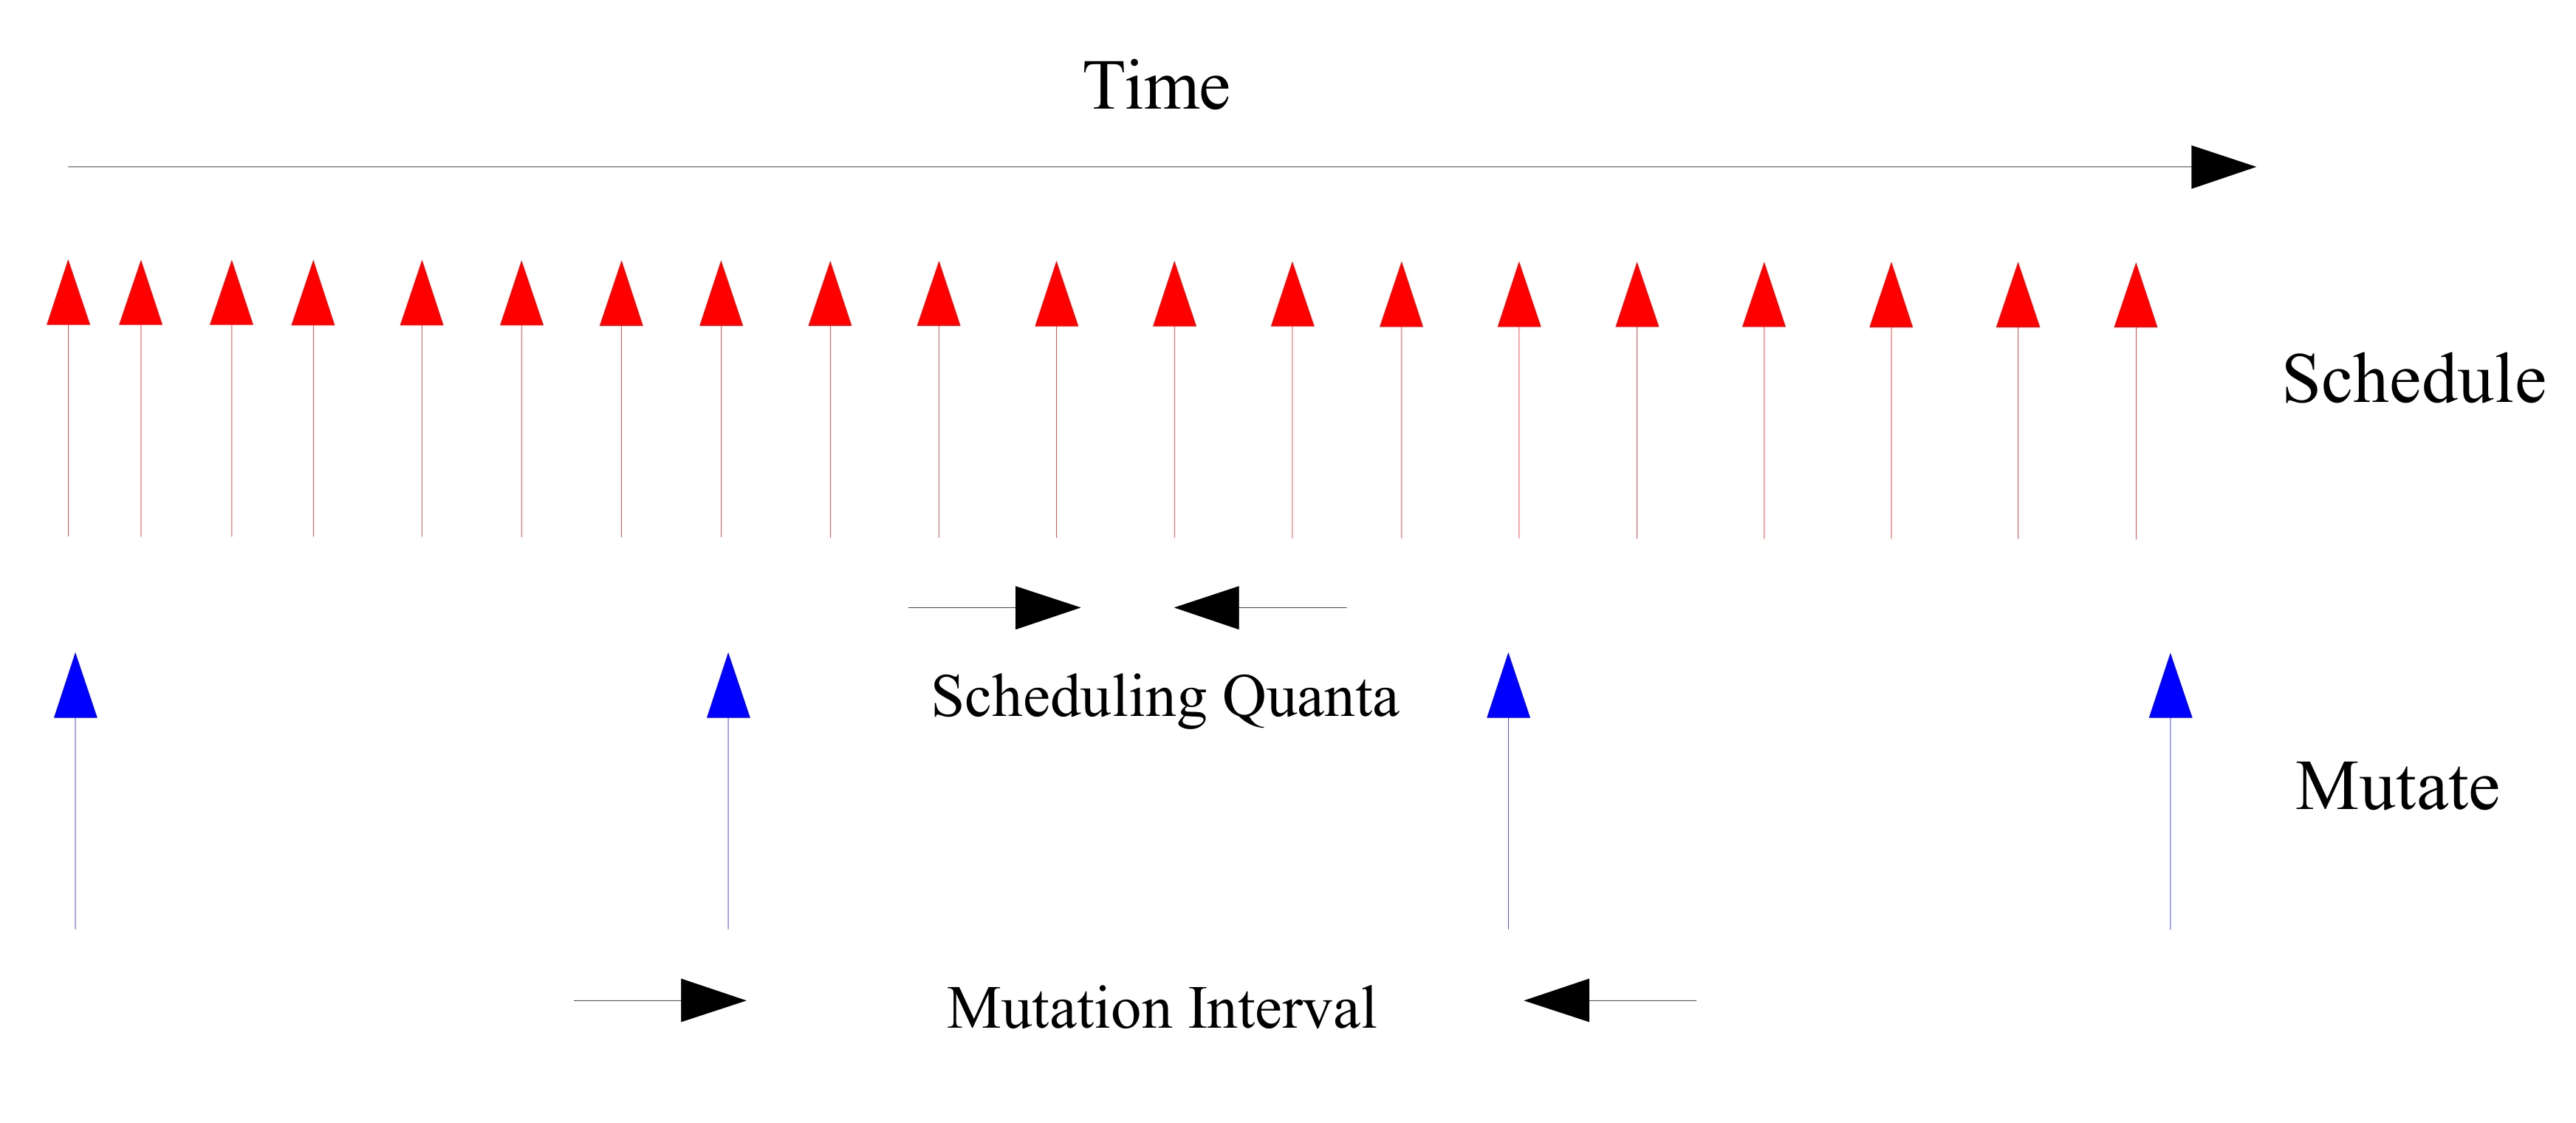
\includegraphics[height=2in]{figures/Schedule_Mutate.jpg}
    \caption{Hypothetical time line displaying the invocation frequencies of the scheduler and the mutator}
    \label{fig:schedule_mutate}
  \end{center}
\end{figure}


Delta ($\Delta$) for a system with \textit{N} processors where each processor \textit{i} is transitioned
from performance state $P_{i}$ to $P_{i}'$ can be defined as shown below in Equation~\eqref{eq:Delta_def}
\begin{equation}
    \Delta \geq \displaystyle\sum_{i=0}^{N-1} {| P_{i} - P_{i}' |}
\label{eq:Delta_def}
\end{equation}
and can also be defined as the Manhattan distance between the layout vector $L$ before the transition and 
the layout vector $L'$ after the transition. Thus the example mutation as shown in Figure~\ref{fig:ex_mutation}
is allowed only for a system with a delta constraint $\Delta \geq 3$. 

\begin{figure}[h!]
  \begin{center}
    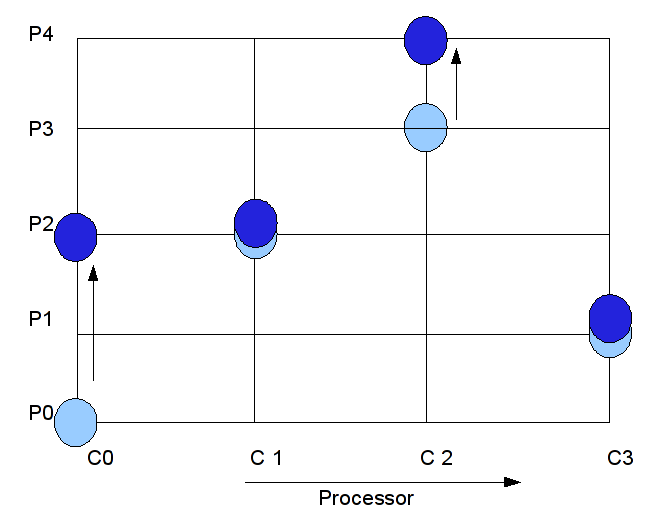
\includegraphics[height=2in]{figures/example_mutation_3.png}
    \caption{Example mutation}
    \label{fig:ex_mutation}
  \end{center}
\end{figure}



%%%%%%%%%%%%%%%%%%%%%%%%%%%%%%%%%%%%%%%%%%%%%%%%%%%%%%%%%%%%%%%%%%%%%%%%%%%%%%%
\section{Problem definition}~\label{sec:ago}
%%%%%%%%%%%%%%%%%%%%%%%%%%%%%%%%%%%%%%%%%%%%%%%%%%%%%%%%%%%%%%%%%%%%%%%%%%%%%%%

An overview of the system required is as follows:
\begin{enumerate}
\item The scheduler estimates the required performance state for each task and maintains the demand, 
a monotonically increasing count, representing the number of times each state was requested. 
\item Each processor can take performance states from $0$ to $M-1$. 
\item The total movements: the Manhattan distance from the current layout to the next layout 
should always be less than or equal to the delta constraint ($\Delta$). 
\item The system should be partial to maintaining a processors current performance state if such a performance state is requested.
\end{enumerate}

This problem can be expressed as a Multiple choice knapsack problem as shown in Figure~\ref{fig:mckp}, where the capacity of the knapsack 
is equal to the delta constraint. Each processor being a variable and multiple choices being the states 
a processor can take. The weight for each choice is the distance that state is from the current 
performance state of the processor. It is well understood that such problems are considered NP-Hard.

\begin{figure}[h!]
\centering
\begin{align*}
    & max \displaystyle\sum_{i=0}^{N-1} \displaystyle\sum_{j=0}^{M-1} d_jx_{ij} \\
    & \text{Subject to} : \displaystyle\sum_{i=0}^{N-1} \displaystyle\sum_{j=0}^{M-1} |L_i - j| x_{ij} \leq \delta \\
    & \displaystyle\sum_{j=0}^{M-1} x_{ij} = 1 , i = 0, 1, ..., N-1 \\
    & x_{ij} \in \{0,1\} , i = 0,1,2,...,N-1 ; j = 0,1,2,...,M-1  
\end{align*}
\caption{Problem with N processors each having M states expressed as a multiple choice knapsack problem}
\label{fig:mckp}
\end{figure}

The algorithm provided in \cite{mckp} was implemented and it soon became obvious 
that the algorithm was inefficient for having no concept of transition direction. Thus for 
a delta constraint of 1, if 
the first 3 processors of a quad core system are at state 0 (The lowest performance state),
while the remaining processor is at state 4 (The highest performance state) and the scheduler
demands all the processors to be at state 3: The dynamic programming approach depicted in
\cite{mckp} will transition the forth processor from state 4 to 3 rather than transition 
one of the lower processors closer to state 3. This unfortunately was just one of the examples
among many when the system did not work. This motivated the development of an iterative 
direction based greedy algorithm described below.


%%%%%%%%%%%%%%%%%%%%%%%%%%%%%%%%%%%%%%%%%%%%%%%%%%%%%%%%%%%%%%%%%%%%%%%%%%%%%%%
\section{The delta constrained mutation algorithm}~\label{sec:delta_algo}
%%%%%%%%%%%%%%%%%%%%%%%%%%%%%%%%%%%%%%%%%%%%%%%%%%%%%%%%%%%%%%%%%%%%%%%%%%%%%%%

Figure~\ref{fig:mutation_algo} describes the steps involved in the iterative greedy algorithm. 
Each sub step is described in further sections. The initialization procedure is described in Section~\ref{sec:mut_init}.
Based on the iteration delta constraint $\delta$, a matrix, Manhattan
matrix (\textbf{S}) is constructed and described in Section~\ref{sec:delta_matrix}.
The Manhattan weight vector \textbf{W} is described in Section~\ref{sec:weight}.
The cooperative demand transformation (Creation of the demand field) is described in
\ref{sec:field}. The greedy winning state \textit{w} selection is described in Section~\ref{sec:winner_state}.
The selection of the processor \textit{c} to transition to the winning state \textit{w} 
is described in Section~\ref{sec:winner_proc}. Finally, the parameter adjustments and iteration
termination conditions are described in Section~\ref{sec:param_adjust}. 

\begin{figure}[h!]
  \begin{center}
    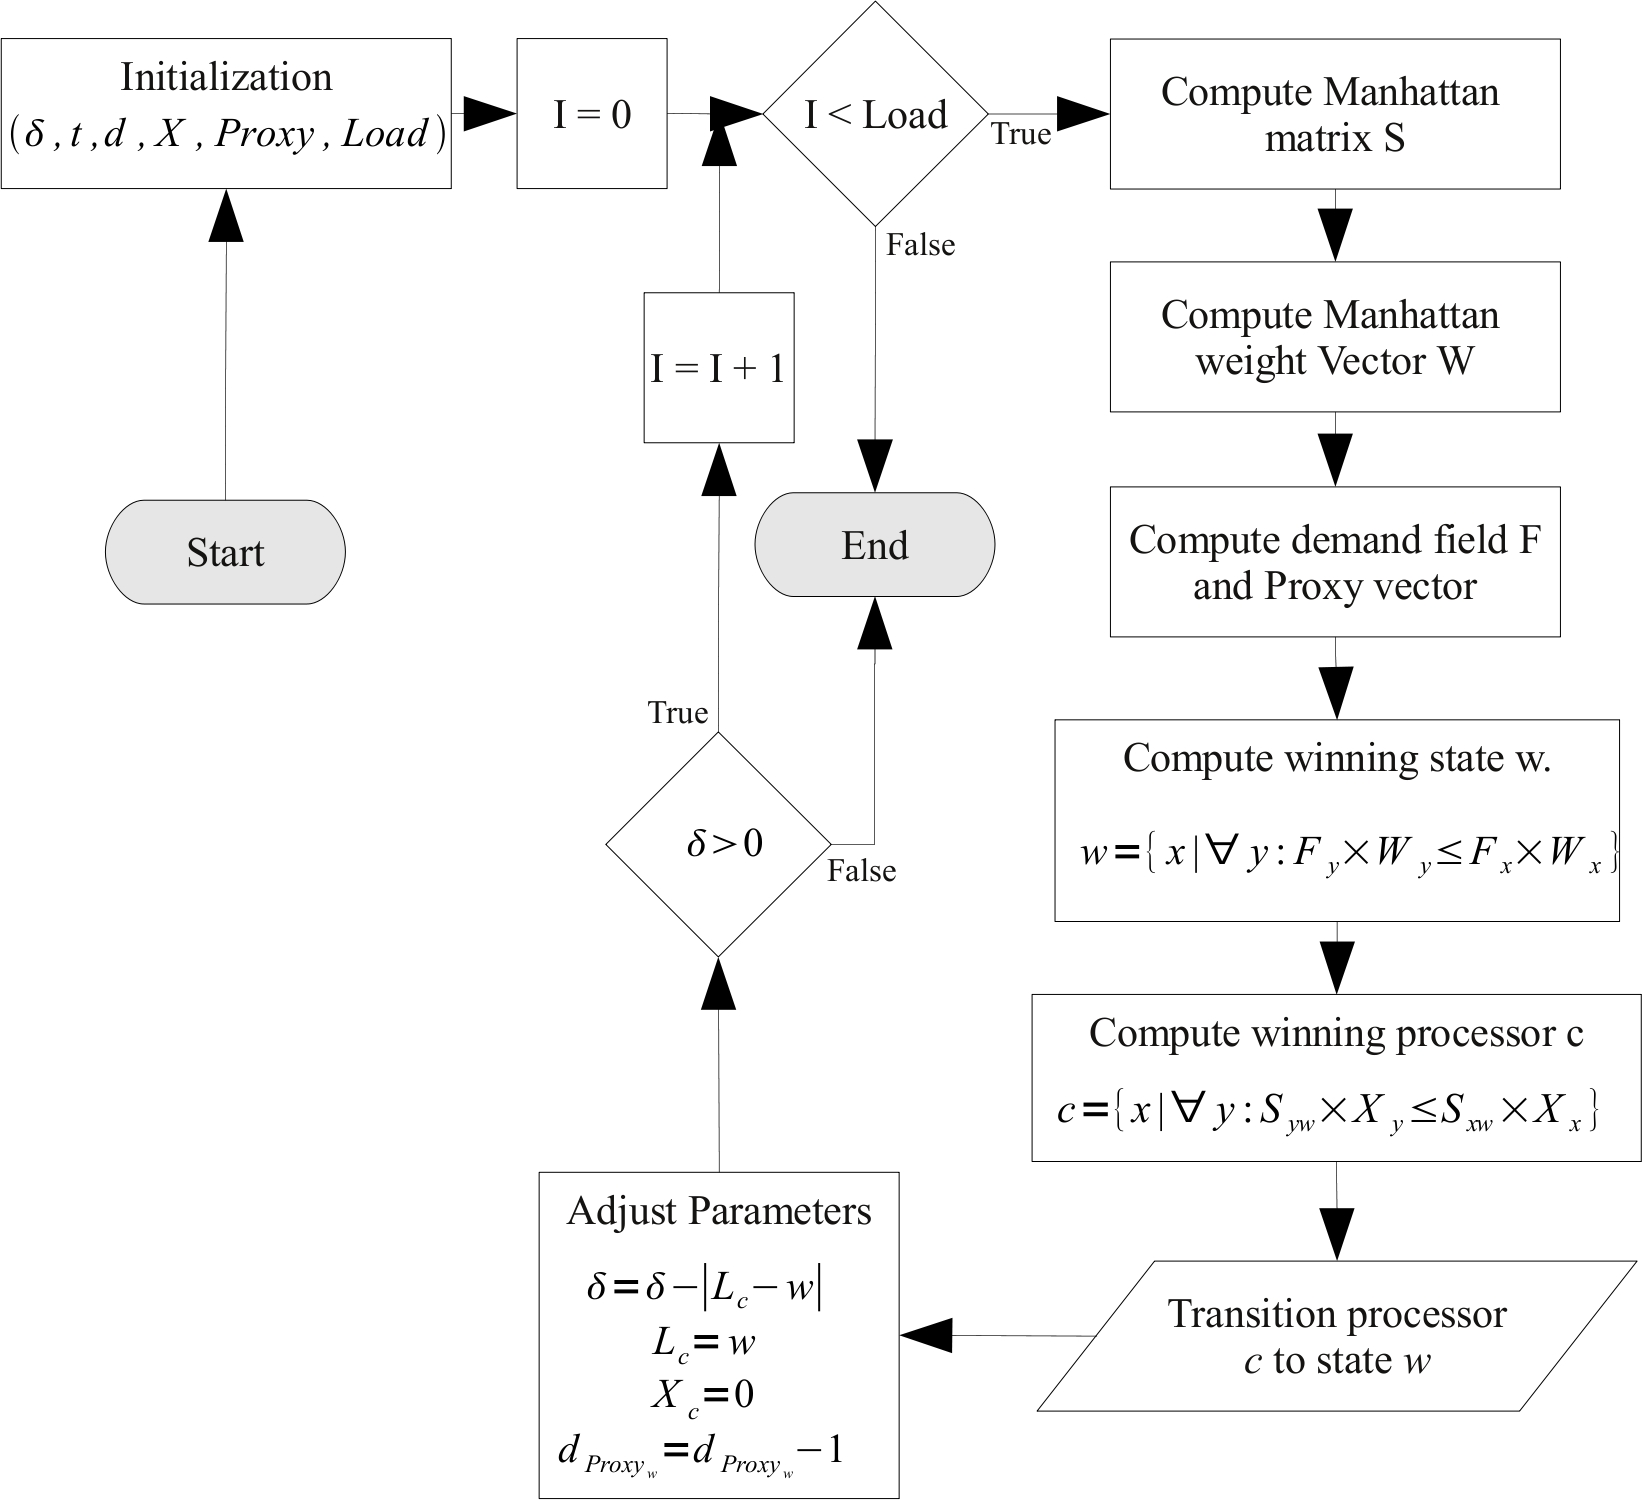
\includegraphics[height=4in]{figures/Mutation_algo.jpg}
    \caption{Mutation algorithm}
    \label{fig:mutation_algo}
  \end{center}
\end{figure}

%%%%%%%%%%%%%%%%%%%%%%%%%%%%%%%%%%%%%%%%%%%%%%%%%%%%%%%%%%%%%%%%%%%%%%%%%%%%%%%
\subsection{Initialization}~\label{sec:mut_init}
%%%%%%%%%%%%%%%%%%%%%%%%%%%%%%%%%%%%%%%%%%%%%%%%%%%%%%%%%%%%%%%%%%%%%%%%%%%%%%%

In order to effectively provide only the needed number of processors, the mutator
queries the operating system for the total number of tasks in the ready state $T$. 
From which, the Load of the system in terms of number of processors required is computed 
as shown below in Equation~\eqref{eq:projected_load},
\begin{equation}
    Load = \left\{
     \begin{array}{lr}
       T & : T \leq N\\
       N & : T > N
     \end{array}
   \right.
\label{eq:projected_load}
\end{equation}
where $T$ is the total number of tasks in the ready state in a multi-processor system with \textit{N} online processors.
Using an estimated load based on idle times
of processors was found to be unfruitful as it can be non-representative of the actual 
computing capacity demanded by the number of active tasks. This can be emphasized in situations where multiple
tasks could be queued on a single processor.

The Performance Directed Scheduler as described in Chapter~\ref{chap:pds} maintains
the demand for each state in the demand vector \textbf{D}. The contents of this vector
cannot be directly consumed as their values pose no direct description of the demand 
of individual performance states. As a direct consequence, vector \textbf{d} is computed based 
on the projected load of the system and the demand vector \textbf{D} shown below in Equation~\eqref{eq:processor_demand},
\begin{equation}
    d_{i} = \frac{D_{i} \times Load}{\displaystyle\sum_{j=0}^{M-1} {D_{j}}}
\label{eq:processor_demand}
\end{equation}
where $D_i$ is the total number of times performance state $P_i$ was requested by the performance directed scheduler in 
the previous mutation interval while the total load of the system was estimated to be \textit{load}. The vector \textbf{d}
is also reffered to as the processor demand as each element $d_i$ is the total number of processors demanded by the 
performance directed scheduler in state $P_i$. 

$Z_P$ the present or current power number of the multi-processor system is computed as shown below in Equation~\eqref{eq:Z_P},
\begin{equation}
    Z_{P} = \displaystyle\sum_{i=0}^{N-1} {L_{i}} 
\label{eq:Z_P}
\end{equation}
where \textit{N} is the total number of online processors and \textbf{L} is the current layout of the system. Thus $Z_P$ 
is an integer value proportional to the total power drawn by the multi-processor system. $Z_R$, the required power number  is computed based on the 
processor demand \textbf{d} as shown below in Equation~\eqref{eq:Z_R},
\begin{equation}
    Z_{R} = \displaystyle\sum_{i=0}^{M-1} {i \times d_{i}} 
\label{eq:Z_R}
\end{equation}
where, each processor is capable of \textit{M} performance states and $d_i$ being the total number of processors demanded
by performance state $P_i$. Thus $Z_R$ is proportional to the power drawn by the multi-processor system when the processors
are transitioned in such a way as to satisfy the performance directed scheduler to optimally assign current tasks. 

Based on $Z_{P}$ and $Z_{R}$, the transition direction, \textit{t}, a tri-state value describing the nature of 
mutation required is computed as shown below in Equation~\eqref{eq:transition_dir}. 
\begin{equation}
    t = \left\{
     \begin{array}{lr}
       1 & : Z_{R} > Z_{P}\\
       0 & : Z_{R} = Z_{P} \\
       -1 & : Z_{R} < Z_{P}
     \end{array}
   \right.
\label{eq:transition_dir}
\end{equation}
A transition direction of $t = +1$ implies that the scheduler requires higher performance from
the multi-processor, while a transition direction of $t = -1$ implies the exact opposite; an indication
to conserve power by reducing the performance states of the multi-processor. A transition direction equal to zero
implies stability and and mutations must be avoided if possible. 

Before starting the iterations, the poison vector \textbf{X} of length \textit{N} is initialized to all ones, where
each element corresponds to a processor. Each element of the poison vector is a binary element with a value of 0 
implying that the processor has been allocated a performance state and must not be re-transitioned, The initialization
of the poison vector is described below in Equation~\eqref{eq:poison_init} for a multi-processor system with \textit{N} processors.
\begin{equation}
    \forall i : 0 \geq i < N; X_{i} = 1 
\label{eq:poison_init}
\end{equation}
The iteration delta constraint $\delta$ is initialized to $\Delta$  ($\delta = \Delta$). 

%%%%%%%%%%%%%%%%%%%%%%%%%%%%%%%%%%%%%%%%%%%%%%%%%%%%%%%%%%%%%%%%%%%%%%%%%%%%%%%
\subsection{The Manhattan matrix}~\label{sec:delta_matrix}
%%%%%%%%%%%%%%%%%%%%%%%%%%%%%%%%%%%%%%%%%%%%%%%%%%%%%%%%%%%%%%%%%%%%%%%%%%%%%%%

The Manhattan matrix \textbf{S} of dimension $N \times M$, can be viewed as a probability matrix where each element
$S_{ij}$ indicates the probability that processor \textit{i} can be transitioned to
performance state \textit{j} for a system with \textit{N} processors each 
capable of \textit{M} transition states. The conception of this matrix was achieved by viewing
a probability density function for each processor and was soon modified due to the lack of floating point operations in kernel space 
(Even though possible, the kernel address space does not save the floating point 
context and makes it's use dangerous as the kernel is fully preempt-able).

The Manhattan matrix ($N \times T$) is computed as shown below (Equation~\eqref{eq:delta_mat}),
\begin{equation}
    \forall i,j \in \mathbb{N} : i < N, j < M; S_{ij} = \left\{
     \begin{array}{lcr}
       0 & : & j < (L_{i} - \delta) \\
       \frac{M}{2} \times (t^{2} - t + 2) + j - L_{i} & : & (L_{i} - \delta) \leq j < L_{i} \\
       2M & : & j = L_{i}\\
       \frac{M}{2} \times (t^{2} + t + 2) - j + L_{i} & : & L_{i} < j \leq (L_{i} + \delta) \\
       0 & : & j > (L_{i} + \delta)
     \end{array}
   \right.
\label{eq:delta_mat}
\end{equation}
where, $L_i$ is the current performance state of processor \textit{i} in a multi-processor enviornment 
with a total of \textit{N} processors each processor capable of \textit{M} performance states 
and the transition direction \textit{t} estimated to be either $-1$, $0$ or $+1$. 

Each row in the Manhattan matrix corresponds to an on-line processor core while each column corresponds to a performance state
in increasing order. Thus $S_{23}$ describes the weight of processor $C_2$ transitioning to the performance state $P_3$. 
For example, consider a hypothetical multiprocessor with a total of 4 processors ($N = 4$) each capable of
5 performance states ($M = 5$) with the current layout \textbf{L} = [0,1,2,3], implying that processors $C_0$, $C_1$, $C_2$ and $C_3$
are in performance states $P_0$, $P_1$, $P_2$ and $P_4$ respectively. 

Based on the processor demand, if the transition direction $t = 1$, implying higher required performance
out of the multi-processor system, and the iteration delta constraint $\delta = 2$, then the Manhattan matrix \textbf{S} 
is shown below (Equation~\eqref{eq:ex_dmuth}).
\begin{equation}
    S^{t = +1} = \left[
     \begin{array}{ccccc}
       10 & 9 & 8 & 0 & 0 \\
       4 & 10 & 9 & 8 & 0 \\
       3 & 4 & 10 & 9 & 8 \\
       0 & 3 & 4 & 10 & 9
     \end{array}
   \right]
\label{eq:ex_dmuth}
\end{equation}
The following can be observed about this matrix (Equation~\eqref{eq:ex_dmuth}):
\begin{enumerate}
\item For each row, \textit{i}, the highest weight of $2M$ (10), is assigned to the element $S_{ij}$ when $j = L_i$. Thus, as $L_0 = 0$, the element $S_{00} = 10$.
\item For each row, \textit{i}, elements $S_{ij}$ are assigned a value of 0, when they are more that $\delta$ elements away ($|j - L_i| > \delta$). Thus elements $S_{03}$ and $S_{04}$
are assigned a value of 0.
\item For each row, \textit{i}, and column $L_i < j \leq (L_i + \delta)$, integer values are assigned to $S_{ij}$ such that they are in decreasing order starting from $2M-1$ (9).
Thus $S_{01}$, $S_{02}$ are given values 9 and 8 respectively. 
\item For each row, \textit{i}, and column $(L_i - \delta) \leq j < L_i$, integer values are assigned to $S_{ij}$ such that they are in decreasing order starting from $M-1$ (4).
Thus $S_{21}$ and $S_{20}$ are given values 4 and 3 respectively.
\end{enumerate}
This construction for a transition direction $t = 1$ favors transitions towards higher performance states. 

For the same example of $N = 4$, $M = 5$, $\delta = 2$ and finally $L = [0,1,2,3]$, the Manhattan matrix \textbf{S} for a transition direction $t = 0$ is shown below (Equation~\eqref{eq:ex_dmut0}).
\begin{equation}
    S^{t = 0} = \left[
     \begin{array}{ccccc}
       10 & 4 & 3 & 0 & 0 \\
       4 & 10 & 4 & 3 & 0 \\
       3 & 4 & 10 & 4 & 3 \\
       0 & 3 & 4 & 10 & 4
     \end{array}
   \right]
\label{eq:ex_dmut0}
\end{equation}
The following can be observed about this matrix (Equation~\eqref{eq:ex_dmut0}):
\begin{enumerate}
\item For each row, \textit{i}, the highest weight of $2M$ (10), is assigned to the element $S_{ij}$ when $j = L_i$. Thus, as $L_0 = 0$, the element $S_{00} = 2 \times 5$.
\item For each row, \textit{i}, elements $S_{ij}$ are assigned a value of 0, when they are more that $\delta$ elements away ($|j - L_i| > \delta$). Thus elements $S_{03}$ and $S_{04}$
are assigned a value of 0.
\item For each row, \textit{i}, and column $L_i < j \leq (L_i + \delta)$, integer values are assigned to $S_{ij}$ such that they are in decreasing order starting from $M-1$ (4).
Thus $S_{01}$, $S_{02}$ are given values 4 and 3 respectively. 
\item For each row, \textit{i}, and column $(L_i - \delta) \leq j < L_i$, integer values are assigned to $S_{ij}$ such that they are in decreasing order starting from $M-1$ (4).
Thus $S_{21}$ and $S_{20}$ are given values 4 and 3 respectively.
\end{enumerate}
This construction for a transition direction $t = 0$ favors transitions in either direction equally. 

Finally, the Manhattan matrix for a transition direction $t = -1$ is shown below (Equation~\eqref{eq:ex_dmutl}).
\begin{equation}
    S^{t = -1} = \left[
     \begin{array}{ccccc}
       10 & 4 & 3 & 0 & 0 \\
       9 & 10 & 4 & 3 & 0 \\
       8 & 9 & 10 & 4 & 3 \\
       0 & 8 & 9 & 10 & 4
     \end{array}
   \right]
\label{eq:ex_dmutl}
\end{equation}
The following can be observed about this matrix (Equation~\eqref{eq:ex_dmutl}):
\begin{enumerate}
\item For each row, \textit{i}, the highest weight of $2M$ (10), is assigned to the element $S_{ij}$ when $j = L_i$. Thus, as $L_0 = 0$, the element $S_{00} = 2 \times 5$.
\item For each row, \textit{i}, elements $S_{ij}$ are assigned a value of 0, when they are more that $\delta$ elements away ($|j - L_i| > \delta$). Thus elements $S_{03}$ and $S_{04}$
are assigned a value of 0.
\item For each row, \textit{i}, and column $L_i < j \leq (L_i + \delta)$, integer values are assigned to $S_{ij}$ such that they are in decreasing order starting from $M-1$ (4).
Thus $S_{01}$, $S_{02}$ are given values 4 and 3 respectively. 
\item For each row, \textit{i}, and column $(L_i - \delta) \leq j < L_i$, integer values are assigned to $S_{ij}$ such that they are in decreasing order starting from $2M-1$ (9).
Thus $S_{21}$ and $S_{20}$ are given values 9 and 8 respectively.
\end{enumerate}
This construction for a transition direction $t = -1$ favors transitions which reduce the performance state of each processor. 


%%%%%%%%%%%%%%%%%%%%%%%%%%%%%%%%%%%%%%%%%%%%%%%%%%%%%%%%%%%%%%%%%%%%%%%%%%%%%%%
\subsection{The Manhattan weight vector}~\label{sec:weight}
%%%%%%%%%%%%%%%%%%%%%%%%%%%%%%%%%%%%%%%%%%%%%%%%%%%%%%%%%%%%%%%%%%%%%%%%%%%%%%%

The Manhattan weight vector $W$ is constructed as shown below (Equation~\ref{eq:state_weight}),
\begin{equation}
    \forall j \in \mathbb{N} : j < M; W_j = \displaystyle\sum_{i=0}^{N-1} {S_{ij}}
\label{eq:state_weight}
\end{equation}
where \textit{N} is the total number of processors and \textit{M} is the total number of
performance states each processors is capable of.
The Manhattan weight vector is achieved by summing along each column 
of the Manhattan matrix and hence providing an insight of the locality of each state. A higher value of $W_i$ 
indicates a higher probability that there exists active processors in or around
performance state \textit{i}, while a null value, $W_i = 0$ indicates that the performance state \textit{i}
can never be achieved under the current delta constraint. 


%%%%%%%%%%%%%%%%%%%%%%%%%%%%%%%%%%%%%%%%%%%%%%%%%%%%%%%%%%%%%%%%%%%%%%%%%%%%%%%
\subsection{Cooperative demand distribution: The demand field}~\label{sec:field}
%%%%%%%%%%%%%%%%%%%%%%%%%%%%%%%%%%%%%%%%%%%%%%%%%%%%%%%%%%%%%%%%%%%%%%%%%%%%%%%

With lower values of $\Delta$, there is a possibility that a state \textit{i},
could be requested with a high demand $d_i$ but due to the current layout and 
delta constraint, have a Manhattan weight $W_i = 0$, implying that a processor 
in performance state \textit{i} can never be provided.
Thus a method was developed in transforming the demand vector \textbf{d}
in such a way that such null performance states cooperatively give up their demand
to the performance state closest to them which has a possibility of being selected. 
This procedure is described in Algorithm~\ref{fig:field}.


\begin{algorithm}[h!]
 \SetLine
 \KwIn{Demand vector \textbf{d}, Manhattan weight vector \textbf{W}}
 \KwOut{Demand field \textbf{F}, Proxy vector \textbf{Proxy}}
 \ForEach{Performance state $i$}{
     $Proxy_i = i$ \;
     $F_i = d_i$ \;
 }
 \ForEach{Performance state $i$}{
   \If{$W_i = 0$ and $d_i > 0$}{
      \If{$t = 1$}{
        $f = max \{ x : x \in N \wedge x < i \wedge W_x > 0 \}$ \;
      }
      \If{$t = -1$}{
        $f = min \{x : x \in N \wedge x > i \wedge W_x > 0 \}$ \;
      }
      \If{$t = 0$}{
        $f = x : x \in N \wedge x \approx i \wedge W_x > 0$ \;
         f is closest to i such that weight $W_f > 0$.
      }
      $F_f = F_f + F_i$ \;
      $F_i = 0$ \;
      $Proxy_f = i$ \;
    }
 }
\caption{Demand field computation}
\label{fig:field}
\end{algorithm}

The demand field \textbf{F} is essentially a replicate of \textbf{d}, and differs under
circumstances when for a particular performance state \textit{i}, $W_i = 0$ and $d_i > 0$,
then its demand is distributed to a friend \textit{f} which varies based on the transition
direction t. If transition direction $t = 1$, then the demand is given to the state \textit{f} closest and lesser than
\textit{i} with $W_f > 0$. If the transition direction $t = -1$ then a friend is searched in 
the opposite direction with $W_f > 0$. Finally when $t = 0$, the closest state \textit{f} to \textit{i} with $W_f > 0$ is chosen as the 
friend. Once the friend state \textit{f} is computed, all the demand $d_i$ is transferred \textit{f}.
In order to track contributions from others, a vector \textbf{Proxy} is maintained indicating 
the source of the demand. Under normal circumstances, $Proxy_i = i$. 

%%%%%%%%%%%%%%%%%%%%%%%%%%%%%%%%%%%%%%%%%%%%%%%%%%%%%%%%%%%%%%%%%%%%%%%%%%%%%%%
\subsection{Greedy performance state selection}~\label{sec:winner_state}
%%%%%%%%%%%%%%%%%%%%%%%%%%%%%%%%%%%%%%%%%%%%%%%%%%%%%%%%%%%%%%%%%%%%%%%%%%%%%%%

Once \textbf{W} and \textbf{F} are computed, performance state \textit{w} is selected
as the winning state when the value of the product $W_w \times F_w$ is the maximum 
for all states \textit{i} and hence reacting to demand and maintaining locality. 
The procedure is mathematically depicted below (Equation~\eqref{eq:winning_state}),
\begin{equation}
    w = {x | \forall y, y \in \mathbb{N} \wedge 0 \leq y < M : W_y \times F_y \leq W_x \times F_x}
\label{eq:winning_state}
\end{equation}
where, \textit{N} is the total number of processors and \textit{M} is the number of
performance states each processor is capable of.

%%%%%%%%%%%%%%%%%%%%%%%%%%%%%%%%%%%%%%%%%%%%%%%%%%%%%%%%%%%%%%%%%%%%%%%%%%%%%%%
\subsection{Greedy processor selection and transition}~\label{sec:winner_proc}
%%%%%%%%%%%%%%%%%%%%%%%%%%%%%%%%%%%%%%%%%%%%%%%%%%%%%%%%%%%%%%%%%%%%%%%%%%%%%%%

With the winning performance state selected, the processor to be transitioned
is determined by the row \textit{c} in the Manhattan matrix whose value $S_{cw} \times X_c$ 
is maximum and shown below (Equation~\ref{eq:winning_proc}). 
\begin{equation}
    c = {x | \forall y, y \in \mathbb{N} \wedge 0 \leq y < N : S_{yw} \times X_y \leq S_{xw} \times X_x}
\label{eq:winning_proc}
\end{equation}

Once the selection is made, processor \textit{c} is transitioned to performance state
\textit{w} by invoking the seeker cpufreq governor described in Section~\ref{sec:cpufreq}.


%%%%%%%%%%%%%%%%%%%%%%%%%%%%%%%%%%%%%%%%%%%%%%%%%%%%%%%%%%%%%%%%%%%%%%%%%%%%%%%
\subsection{Parameter change and termination conditions}~\label{sec:param_adjust}
%%%%%%%%%%%%%%%%%%%%%%%%%%%%%%%%%%%%%%%%%%%%%%%%%%%%%%%%%%%%%%%%%%%%%%%%%%%%%%%

At the end of every iteration, the parameters $\delta$, $L_c$ and $d_p$ are updated
to represent the transition. First as a transition was previously performed, the iteration delta constraint
must reduce by an equal order as shown below (Equation~\eqref{eq:update_delta}).
\begin{equation}
    \delta = \delta - |L_{c} - w| 
\label{eq:update_delta}
\end{equation}
Second, as processor \textit{c} is no longer in performance state $L_c$, it is updated to
it's new value \textit{w} as shown below (Equation~\eqref{eq:update_L}) 
\begin{equation}
    L_{c} = w 
\label{eq:update_L}
\end{equation}
Third, as a processor is assigned to performance state \textit{w},
the corresponding demand can be reduced as shown below (Equation~\eqref{eq:update_d}).
\begin{equation}
    d_{Proxy_w} = d_{Proxy_w} - 1 
\label{eq:update_d}
\end{equation}
Note that, due to the distortion introduced by the cooperative demand distribution, $d_{Proxy_w}$ is updated
instead of $d_w$. 
Lastly, the poison vector's position for processor
\textit{c} is set to zero and hence disabling processor \textit{c} in participating in a future transition as shown
below (Equation~\eqref{eq:update_X}).
\begin{equation}
    X_c = 0
\label{eq:update_X}
\end{equation}

This concludes a single iteration of the greedy direction based algorithm and is repeated for \textit{Load} iterations
as long as the iteration delta constraint $\delta > 0$. The upper bound on the number of iterations is obviously \textit{Load} 
and ensures early termination of the iterative algorithm when unnecessary.



